% Define the document class:
\documentclass[12pt, a4paper, twoside]{report}
\setcounter{secnumdepth}{4}
%import packages
\usepackage{datetime}
\newdateformat{monthyeardate}{\monthname[\THEMONTH] \THEYEAR}
\usepackage{graphicx} % for images
\usepackage{natbib} % for citation
\bibliographystyle{ctrH} % custom Cite Them Right Harvard referencing
\renewcommand{\bibname}{References} % change name of Bibliography to References
\usepackage{setspace} % allow line spacing to be defined
\onehalfspacing
\setlength{\parindent}{0pt}
\setlength{\parskip}{0.5\baselineskip}
\usepackage[left=2cm, right=2cm, bottom=2.5cm, top=2cm]{geometry} %define margines
\usepackage{textcomp} % for additional fonts and symbols
\usepackage{tabularx} % for tables
\usepackage{array}
\usepackage{enumitem} % for numbered lists
\setlist{topsep=3pt, partopsep=0pt, parsep=0pt, itemsep=0pt}
\usepackage{amssymb} % for additional fonts and symbols
\usepackage{acronym} % for list of acronyms
\usepackage{longtable}
\usepackage{hyperref}
\usepackage{float}
\raggedbottom

\title{Post-MDT Oncology Workflow Bottlenecks: A Design-Science Study of an NHS Integrated Data Repository and Decision-Support Dashboard to Reduce Delays from MDT Outcome to Treatment Start}
\author{Mark Collins}
\date{\today}

\begin{document}

% Title Page
\begin{titlepage}
    \centering
    \vspace*{1cm}
    % Logo
    
\includegraphics[width=0.25\textwidth]{logo.png}\\
    \vspace{1cm}
    {\Large University of Essex Online\par}
    \vspace{1.5cm}
    {\LARGE\bfseries Post-MDT Oncology Workflow Bottlenecks: \par}
    \vspace{0.6cm} 
    {\large A Design-Science Study of an NHS Integrated Data Repository and Decision-Support Dashboard to Reduce Delays from MDT Outcome to Treatment Start. \par}
    \vfill
    {\Large Mark Collins}\par
    \vspace{0.3cm}
    Student ID: 12696434 \par
    \vspace{1cm}
    A dissertation submitted in partial fulfilment of the requirements for the degree of \par
    \vspace{0.3cm}
    \textbf{Master of Science (MSc)} \\ Enterprise IT Management
    \vfill
    {\large Submitted: \monthyeardate\today}
\end{titlepage}

% Front matter
\clearpage
\pagenumbering{roman}


\clearpage 
\phantomsection 
\addcontentsline{toc}{chapter}{Declaration} 
\vspace*{\fill} 
\begin{center} 
    {\bfseries Declaration} 
\end{center} 
\vspace{0.8cm} 

I hereby declare that:
\begin{itemize}
	\item  This is my own work and there is no involvement from a third party. Where someone else’s ideas are used, I have referenced and paraphrased those materials. This includes the use of generative AI tools: where I have used generative AI, I have referenced the tool, stated what it has been used for and given a link to the chat and prompts used. I have read and understood the University of Essex Online Integrity guidelines and declare that this assignment conforms to the rules and regulations. For full details see your Student Handbook (Academic honesty and good academic practice). 
	\item Does not use documentation or data, which is not freely accessible to the public without permission. In addition, where information may identify stakeholders (participants, employees, patients, etc) this has been anonymised. 
\end{itemize}

\begin{flushright}
Mark Collins \\
\monthyeardate\today
\end{flushright}

\vspace*{\fill} 
\clearpage

\begin{abstract}
    Delays between multidisciplinary team (MDT) decision-making and treatment initiation remain a significant challenge within National Health Service (NHS) cancer pathways. Operational data relevant to these workflows are frequently distributed across multiple systems, limiting visibility of bottlenecks and reducing the ability of service managers to intervene proactively. This study applied a Design Science Research (DSR) methodology to design, develop, and evaluate an Integrated Data Repository (IDR) and decision-support dashboard suite for post-MDT oncology pathway management within Portsmouth Hospitals University NHS Trust. 
    
    The artefact integrated oncology referral, outpatient clinic, and radiotherapy datasets using an automated extract-transform-load (ETL) architecture implemented in Python and PostgreSQL. A layered repository design incorporating staging, transformation, and analytics-ready reporting layers was developed to support pathway analysis and operational reporting. Three Power BI dashboards were produced to support referral management, radiotherapy service management, and end-to-end pathway monitoring. 
    
    Analysis of integrated pathway data identified a median post-MDT pathway duration of 37 days. The largest delay occurred between CT simulation and treatment initiation (16 days), followed by the interval between triage and first oncology clinic attendance (8 days). Repository development also identified previously unrecognised operational data-quality issues including duplicate referral records, incomplete clinic outcome recording, and inconsistencies between operational systems. The developed dashboards provided visibility of active pathway risks, radiotherapy capacity utilisation, and operational bottlenecks not readily observable through existing reporting processes. 
    
    The study contributes both a practical artefact and a set of evaluated design principles for operational oncology analytics. Findings demonstrate that meaningful improvements in operational visibility can be achieved through lightweight data integration approaches without replacing existing clinical systems. Future work should focus on integration of structured digital referrals, Systemic Anti-Cancer Therapy (SACT) datasets, clinic-capacity modelling, and further decomposition of treatment-planning workflows.
\end{abstract}

\clearpage 
\phantomsection 
\addcontentsline{toc}{chapter}{Acknowledgements} 
\vspace*{\fill} 
\begin{center} 
    {\bfseries Acknowledgements} 
\end{center} 
\vspace{0.8cm} 

I would like to express my sincere gratitude to my supervisor, Dr. Adrian Euler, for his guidance, encouragement, and constructive feedback throughout this research project. His support and expertise were invaluable in shaping both the direction and quality of this dissertation. 

I am also grateful to colleagues within Portsmouth Hospitals University NHS Trust who generously shared their knowledge and expertise of operational oncology workflows and participated in the evaluation of the developed artefact. Their insights provided essential real-world context and helped ensure the practical relevance of this study. 

Finally, I would like to express my deepest appreciation to my family for their unwavering support, patience, and encouragement throughout the past two years of study. In particular, I am profoundly grateful to my wife, Abi, whose constant belief in me, understanding, and support made the completion of this programme possible. 
\vspace*{\fill} 
\clearpage


\setcounter{tocdepth}{1}
\tableofcontents
\clearpage
\addcontentsline{toc}{chapter}{List of Figures}
\listoffigures
\clearpage
\addcontentsline{toc}{chapter}{List of Tables}
\listoftables
\clearpage
\chapter*{List of Acronyms}
\addcontentsline{toc}{chapter}{List of Acronyms}
\begin{acronym}

\acro{AI}{Artificial Intelligence}

\acro{CDSS}{Clinical Decision Support System}
\acro{CDW}{Clinical Data Warehouse}
\acro{CWT}{Cancer Wait Time}

\acro{DSR}{Design Science Research}
\acro{DSRM}{Design Science Research Methodology}
\acro{DTI}{Diagnosis to Treatment Interval}
\acro{DTT}{Decision-to-Treat}

\acro{ETL}{Extract-Transform-Load}
\acro{EPR}{Electronic Patient Record}

\acro{FDS}{Faster Diagnosis Standard}
\acro{FHIR}{Fast Healthcare Interoperability Resources}

\acro{GDPR}{General Data Protection Regulation}

\acro{HCI}{Human Computer Interaction}
\acro{HR}{Hazard Ratio}

\acro{IDR}{Integrated Data Repository}

\acro{JCCO}{Joint Council for Clinical Oncology}
\acro{JSON}{JavaScript Object Notation}

\acro{MDT}{Multidisciplinary Team}

\acro{NCWTMDS}{National Cancer Waiting Times Monitoring Data Set}
\acro{NHS}{National Health Service}

\acro{OIS}{Oncology Information System}

\acro{PAS}{Patient Administration System}
\acro{PACS}{Picture Archiving and Communication System}
\acro{PDCA}{Plan - Do - Check - Act}
\acro{PTL}{Patient Tracking List}

\acro{QA}{Quality Assurance}

\acro{RCR}{Royal College of Radiologists}
\acro{RIS}{Radiology Information System}
\acro{RTT}{Referral To Treatment}

\acro{SABR}{Stereotactic Ablative Body Radiotherapy}
\acro{SACT}{Systemic Anti Cancer Therapy}
\acro{SQL}{Structured Query Language}
\acro{SUS}{System Usability Scale}

\end{acronym}


% Main matter
\cleardoublepage
\pagenumbering{arabic}

\chapter{Introduction}
Delivering timely cancer care remains a critical priority within the NHS, where delays at any stage of the diagnostic and treatment pathway can negatively affect patient outcomes, experience, and service performance. Recent policy reforms have consolidated the NHS Cancer Waiting Time (CWT) framework into three outcome-focused standards: the 28-day Faster Diagnosis Standard (FDS), the 31-day decision-to-treat to treatment (DTT) standard, and the 62-day referral-to-treatment (RTT) standard—implemented nationally from October 2023 \citep{johnson2024, NHSDigital2026}. These standards place increased emphasis on operational viability, rapid decision-making, and efficient progression of patients through the post-MDT (multidisciplinary team) stages of the oncology pathway. However, many Trusts continue to face systemic challenges in generating timely, accurate, and actionable insights from fragmented data sources.

Within Portsmouth Hospitals University NHS Trust, as in many NHS institutions, key operational data concerning MDT outcomes, clinic scheduling, booking practices, and treatment initiation remain dispersed across siloed systems. Although these systems individually support MDT coordination, outpatient clinic management, and treatment delivery, they lack a consolidated view of pathway performance. This fragmentation makes it difficult for operational managers to detect bottlenecks, identify emerging breach risks, or allocate clinical capacity efficiently. As a result, delays between MDT outcomes, first oncology clinic, decision-to-treat, and first definitive treatment remain insufficiently visible, impairing the Trust's ability to monitor compliance with the 31- and 62-day standards and to respond rapidly to operational pressures.

To address this challenge, the study adopts a Design Science Research (DSR) approach, developing and evaluating an Integrated Data Repository (IDR) and decision-support dashboard suite intended to improve operational visibility of post-MDT oncology workflows.

\section{Problem Statement}

The central problem addressed in this research is the absence of an integrated, operationally focused data infrastructure and decision-support interface to illuminate post-MDT workflow delays and guide timely interventions within an NHS oncology service. Despite the availability of relevant data, the lack of integration and harmonisation across MDT, clinic, and treatment systems results in manual workarounds, inconsistent performance monitoring, and delayed insights. This gap diminishes the ability of operational teams to identify patients at risk of breaching national cancer standards, understand the factors driving variability in pathway intervals, and proactively manage capacity-constrained environments.

Moreover, existing reporting solutions tend to focus on aggregate compliance metrics after the fact, rather than providing real-time or near-real-time visibility of operational bottlenecks. Without a unified source of truth that aligns event definitions, timestamps, and clinical coding standards \citep{NHSDigital2026}, it becomes difficult to execute performance analysis or support day-to-day decision-making. Literature on Integrated Data Repositories (IDRs) similarly highlights that many institutions struggle with data harmonisation, terminological alignment, and the creation of analytics-ready architectures capable of supporting both research and operational use cases \citep{gagalova2020}.

This study therefore seeks to design, develop, and evaluate a lightweight Integrated Data Repository (IDR) and accompanying decision-support dashboard tailored specifically to the post-MDT oncology workflow. By integrating key pathway events, clinic capacity information, and national standard definitions, the artefact aims to surface bottlenecks, highlight breach risks, and support operational teams in prioritising actions that improve pathway performance.

\section{Research Aim and Objectives}

\subsection{Research Aim}
To design and evaluate an IDR and decision-support dashboard capable of improving operational visibility and proactive management of post-MDT oncology pathways.

\subsection{Objectives}
\begin{enumerate}
    \item Identify and quantify post-MDT pathway delays.
    \item Determine operational factors associated with delay.
    \item Design an integrated data architecture.
    \item Develop a user-centred dashboard.
    \item Evaluate utility, usability, and technical validity.
    \item Derive transferable design principles
\end{enumerate}

\begin{table}[h]
    \centering
    \begin{tabular}{|p{5cm}|p{5cm}|p{5cm}|}
        \hline
        \textbf{Research Question} & \textbf{DSR Activity} & \textbf{Primary Methods} \\
        \hline\hline
        \textbf{RQ1}: Where do delays occur between MDT outcome and treatment? & Problem identification & Descriptive statistics, interval analysis \\
        \hline
        \textbf{RQ2}: What operational factors are associated with delay? & Problem analysis & Descriptive and operational analysis\\
        \hline
        \textbf{RQ3}: Does the artefact improve operational decision-making? & Evaluation & SUS, Stakeholder feedback, Design principle validation\\
        \hline
        \textbf{RQ4}: What design principles support post-MDT operational analytics? & Design knowledge & Literature synthesis and evaluation synthesis\\
        \hline
    \end{tabular}
    \caption{This mapping ensures methodological coherence between the research questions, artefact, and evaluation.}
    \label{tab:rq-dsr-mapping}
\end{table}

\section{Research Approach}

This study adopts Design Science Research (DSR) because the primary objective is not solely to explain an existing phenomenon but to create and evaluate an artefact intended to address an identified organisational problem. Whereas case-study research focuses on understanding contextual factors and Action Research emphasises organisational change through iterative intervention, DSR provides a structured framework for the design, construction and evaluation of innovative technological artefacts while simultaneously generating transferable knowledge \citep{hevner2004, peffers2007}.

The approach is particularly appropriate given the need to integrate heterogeneous operational data sources and translate them into actionable decision support for NHS oncology services. Similar DSR approaches have been successfully applied within health informatics, clinical decision support, and healthcare analytics domains where practical solutions and theoretical contribution are required concurrently \citep{harper2023, johnson2020}.

The study therefore follows the six-stage Design Science Research Methodology (DSRM) proposed by \cite{peffers2007}, with detailed application described in Chapter \ref{method}.

The study contributes both a practical artefact and transferable design knowledge. Practically, it delivers an operationally focused Integrated Data Repository and dashboard suite capable of improving visibility of post-MDT oncology pathways. Academically, it contributes a set of evaluated design principles for operational oncology analytics and demonstrates the application of Design Science Research within an NHS operational setting.  

\section{Academic and Practical Significance}

Academically, the research contributes to the limited body of DSR-grounded studies focusing on NHS operational analytics, offering:
\begin{itemize}
    \item an IDR reference architecture for oncology operations;
    \item a set of design principles for NHS-appropriate decision-support dashboards;
    \item an evaluation protocol combining usability metrics, decision-quality testing, and technical verification.
\end{itemize}

Practically, the artefact provides operational teams with a tool that can:
\begin{itemize}
    \item reduce time-to-insight;
    \item support rapid identification of bottlenecks and breach risks;
    \item align capacity planning with demand;
    \item improve pathway monitoring in line with the 28-, 31-, and 62-day standards.
\end{itemize}

Ultimately, the study aims to support faster, more reliable progression from MDT decision to treatment initiation, with the potential to support improved patient care and more effective management of oncology services.

The completed study identified two principal contributors to pathway duration: the interval between triage and first oncology clinic attendance (8 days) and the interval between CT simulation and treatment initiation (16 days). In addition, repository development revealed previously unrecognised data-quality issues associated with manual administrative processes. These findings demonstrate how integrated operational data can provide insights that were not previously available through existing reporting mechanisms. 

\chapter{Literature Review}

\section{Introduction}

The purpose of this literature review is to synthesise and critically evaluate existing research relevant to the design of an Integrated Data Repository (IDR) and operational analytics dashboard aimed at improving post-MDT oncology pathway efficiency. Timely cancer treatment has profound implications for survival, patient experience, resource utilisation, and system performance. Evidence from national datasets, observational studies, systematic reviews, and informatics research shows that delays between MDT decisions and treatment initiation remain persistent across the NHS. Furthermore, data fragmentation, inconsistent recording practices, and limited visibility of operational bottlenecks hinder the ability of clinicians, MDT coordinators, and service managers to proactively manage these delays.

The review is organised around five interrelated themes:
\begin{enumerate}
    \item MDT operations and evolving pressures on multidisciplinary cancer decision making;
    \item Operational delays across the cancer pathway, particularly diagnosis-to-treatment intervals (DTI);
    \item Data fragmentation and the case for integrated data repositories;
    \item Dashboards and performance-monitoring tools to support operational decision-making;
    \item Emerging data trends and the role of ETL, interoperability, AI and multimodal data integration.
\end{enumerate}

Collectively, this literature forms the conceptual foundation (kernel theory) for the artefact developed in this study. The following sections provide a detailed account of these themes, integrating high-quality evidence from the UK, international datasets, clinical oncology, health informatics, and organisational science.

\subsection{Method}
An iterative literature review was adopted, following the guidance outlined by  \cite{dawson2015} (Figure \ref{fig:LitProc}). An initial search was conducted using Google Scholar and open-access repositories to identify foundational concepts and terminology related to Integrated Data Repositories, cancer pathways, MDT operations, dashboards, and Design Science Research. These preliminary results informed a more structured search strategy applied to ScienceDirect, IEEEXplore, and PubMed.

Searches were limited to peer-reviewed journals, systematic reviews, national audits, and authoritative policy documents published primarily between 2010 and 2026, with earlier seminal works retained where conceptually relevant (e.g. JCCO report \citep{ash2004}, the Calman-Hine report \citep{calman1995} and Design Science Research foundations). Studies were included if they addressed MDT processes, oncology pathway delays, health data integration, dashboards, usability standards, or operational analytics. Articles focused exclusively in molecular biology, single-modality clinical trials, or non-healthcare data systems were excluded. 

Approximately 90 sources were reviewed during the process, with around 55 core studies retained for detailed analysis based on relevance, methodological quality, and applicability to NHS operational contexts. Backward citation tracking was used to identify influential seed papers and ensure conceptual completeness.

\begin{figure}
    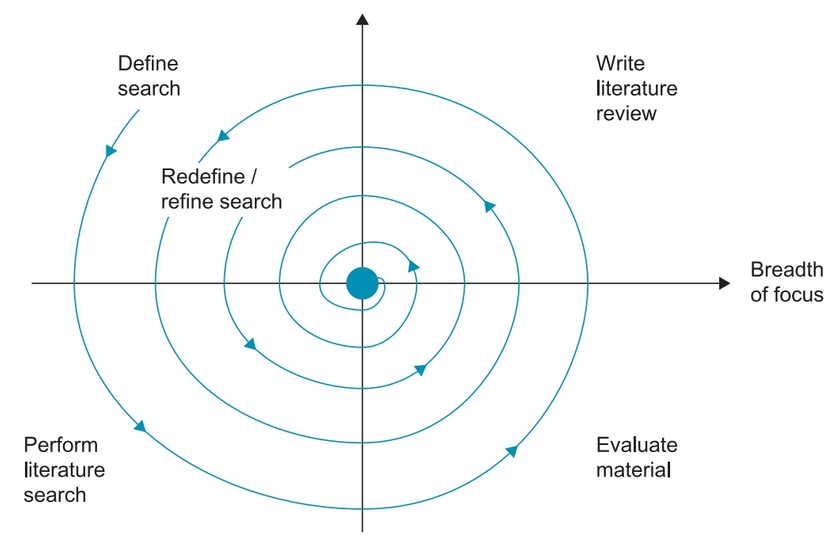
\includegraphics[width=\linewidth]{LitProc.png}
    \caption{Iterative literate review process \citep{dawson2015}}
    \label{fig:LitProc}
\end{figure}

\section{The NHS Cancer Pathway and MDT Framework}

\subsection{MDTs as the Backbone of UK Cancer Care}

Since the publication of the Calman–Hine report \citep{calman1995} and subsequent interventions, MDTs have been embedded as the central governance structure for cancer decision making \citep{haward2006, price2014, morris2006, morris2008}. The MDT model mandates that every new cancer case in the UK is discussed by a multidisciplinary panel including oncologists, surgeons, radiologists, pathologists, specialist nurses, and allied professionals. The 2024 NHS Wales MDT Charter emphasises the crucial role MDTs play in standardising care, reducing unwarranted variation, and improving outcomes by bringing domain experts together in real time \citep{nhswales2024}. Prospective benefits include higher adherence to guidelines, improved communication, shared decision-making, and better coordination of multi-modal treatment plans.

However, the complexity of modern cancer care has increased dramatically alongside rising incidence, new treatment options, biomarker-based stratification, digital imaging volume, and genomic data availability. MDTs now contend with substantially larger case numbers, more complex diagnostic information, and resource pressures that stretch meeting capacity. Professional societies and national audits consistently highlight that MDT meetings are often over-subscribed, under-resourced, and administratively burdensome. These pressures compromise the quality of discussion and create operational bottlenecks that directly affect patient pathways.

\subsection{Evidence of MDT Operational Pressures}

Several studies provide evidence of the challenges affecting MDT functioning:

\begin{itemize}
    \item \cite{soukup2022} conducted a detailed observational analysis of 822 case discussions across three UK MDTs. Administrative and process issues occurred in 30\% of cases, attendance problems in 16\%, and equipment issues in 5\%. These logistical challenges significantly reduced the quality of information and decision-making, demonstrating how operational inefficiencies detract from MDT effectiveness.
    \item \cite{lim2025} analysed 1,488 UK Head and Neck Cancer patients across 50 MDTs and found extremely low compliance with national cancer pathway standards: 32.8\% (FDS), 33.3\% (31‑day), and 34.6\% (62‑day). Median DTT-to-treatment was 42 days.
    \item \cite{chakravarty2023} demonstrated that patients referred from secondary-care outpatient pathways experienced significantly longer delays to MDT discussion and treatment (mean 102 vs. 88 days). These patients were also more likely to receive palliative rather than curative treatment.
    \item \cite{law2024} identified a decade of known MDT barriers including time pressures, communication challenges, inconsistent attendance, information deficits, and increasing clinical complexity.
\end{itemize}

While these studies consistently demonstrate operational strain within MDT processes, several limitations should be acknowledged. Much of the existing evidence is observational and focuses primarily on meeting effectiveness, communication quality, or decision-making processes rather than downstream operational consequences following MDT outcomes.For example, \cite{soukup2022} identify logistical and administrative barriers that impair MDT performance, yet the study does not examine whether these issues translate into measurable delays in treatment initiation. Similarly, the scoping review proposed by \cite{law2024} aggregates a broad range of organisational challenges but provides limited insight into which barriers exert the greatest influence on pathway performance.   

Large-scale cohort studies such as \cite{lim2025} quantify poor compliance with national standards, but their retrospective design offers little visibility of the specific workflow stages responsible for delay accumulation. Consequently, while the literature establishes that MDT processes operate under significant pressure, a gap remains in understanding how operational data can be used to identify, monitor, and mitigate delays arising after MDT decisions have been made. This distinction is important because improving MDT discussion quality alone may be insufficient if subsequent scheduling and treatment processes remain poorly coordinated.

\subsection{National policy direction and waiting time standards}

NHS England's 2024/25 planning guidance emphasises compliance with the Faster Diagnosis Standard (FDS) and cancer treatment timeliness metrics. Persistent waiting-time challenges, data-quality requirements, and the need for integrated pathway oversight tools are highlighted \citep{parker2026}. Radiotherapy services face particular strain: the Royal College of Radiologists reported over 2,300 breaches of the 31‑day standard in October 2023 \citep{rcr2024}. Hidden waits—such as 20‑week delays between surgery and radiotherapy—are not systematically captured, further illustrating limitations in operational visibility.

\section{Operational Delays in Cancer Pathways}

\subsection{Diagnosis-to-Treatment Interval (DTI) as a Critical Metric}

A robust body of literature demonstrates that prolonged DTI adversely affects survival across multiple cancer types.

Key findings include:

\begin{itemize}
    \item \cite{hanna2020}: A systematic review of 34 studies (1.27M patients) found each four-week delay increased mortality by up to 6–8\% across treatment modalities.
    \item \cite{coca-pelaz2018}: Delays in Head and Neck Small Cell Carcinoma beyond four weeks contribute to tumour progression and reduced local control.
    \item \cite{sharma2016}: Delays greater than 30 days reduce overall survival (HR 1.12), with mortality increasing 2.2\% per additional week.
    \item \cite{villemure-poliquin2025}: Treatment within 30 days improves survival by 9\%.
    \item \cite{saleh2024}: Cervical cancer survival drops dramatically after 30 days.
\end{itemize}

\subsection{Hospital/System Factors Influencing Delay}

Large-scale evidence shows that delays are driven not only by tumour characteristics but also by organisational inefficiencies:

\begin{itemize}
    \item \cite{yun2012}: Delays over one month worsened outcomes, especially in low-volume hospitals.
    \item UK audits (e.g., \cite{lim2025}) highlight delays in biopsies, imaging, scheduling, and treatment booking.
\end{itemize}

A further limitation of the current literature is the tendency to treat organisational performance as a static characteristic rather than a dynamic process. Factors such as hospital volume, resource availability, and service configuration are frequently associated with treatment delays; however, there is comparatively little exploration of how these risks evolve over time or how operational teams can intervene before delays become breaches. This reinforces the distinction between retrospective performance measurement and proactive pathway management.

\subsection{MDT-specific drivers of post-decision delays}

\begin{itemize}
    \item Missing diagnostic information and administrative errors cause re-discussion delays \citep{soukup2022}.
    \item High caseloads reduce decision completeness.
    \item Secondary‑care referrals introduce additional diagnostic delays \citep{chakravarty2023}.
    \item Capacity constraints (radiotherapy, theatres, oncology clinics) generate downstream bottlenecks.
\end{itemize}

Although the evidence linking treatment delay and mortality is compelling, caution should be exercised when applying these findings directly to operational improvement initiatives. Most studies evaluate aggregated diagnosis-to-treatment intervals and therefore provide limited insight into the relative contribution of individual pathway stages. While the findings clearly establish delay as clinically important, they do not identify where operational interventions are likely to deliver the greatest benefit. From a service management perspective, this highlights the need for more granular operational analytics capable of decomposing pathway delays into actionable components.

\subsection{Crititcal synthesis of delay literature}

Collectively, the literature provides strong evidence that prolonged diagnosis-to-treatment intervals adversely affect patient outcomes across multiple cancer types. However, important limitations remain when attempting to translate this knowledge into operational practice. Most studies conceptualise delay as a single aggregated interval and consequently offer limited support for identifying specific workflow bottlenecks. Furthermore, while organisational variables such as hospital volume, diagnostic complexity, and service capacity are frequently identified as contributors to delay, relatively little attention has been given to the role of integrated operational data in supporting proactive intervention.

This omission is particularly significant within NHS oncology services, where national performance standards require action before breaches occur. Once a patient has experienced a clinically significant delay, retrospective performance reporting provides little opportunity to prevent harm. Accordingly, there is a need for analytical approaches capable of identifying emerging risks and supporting early operational intervention, rather than simply documenting historical performance.



\section{Data Fragmentation and the Need for Integrated Data Repositories}

\subsection{Fragmentation Across NHS Systems}

Oncology data spans EPRs, PAS, pathology, RIS/PACS, radiotherapy systems, chemotherapy e‑prescribing, Somerset/Cosmic, and MDT spreadsheets.

Evidence includes:

\begin{itemize}
    \item Operational policy from Royal Wolverhampton highlights inconsistent event definitions and PTL challenges \citep{theroyalwolverhamptonnhstrust2024}.
    \item \cite{varma2026}: 92.3\% agreement between CWT and hospital data only when treatment occurs within 100 days; discrepancies arise from definition mismatches and missing fields.
\end{itemize}

\subsection{Clinical Data Warehouses (CDWs) and the Evolution Toward IDRs}

Examples:

\begin{itemize}
    \item ROOT CDW: real‑time repository for 67,000+ cancer patients \citep{jung2021}.
    \item ONCO‑FAIR: chemotherapy‑specific FHIR extensions \citep{guilbert2024}.
    \item NHS–industry multimodal genomic-clinical data lake \citep{conway2025}.
    \item HN‑XNAT: federated imaging and radiotherapy repository \citep{butterworth2025}.
\end{itemize}

While these examples demonstrate the technical feasibility of large-scale oncology data repositories, their transferability to routine NHS operational environments warrants careful consideration. Many reported implementations originate from digitally mature organisations with substantial informatics capability, dedicated technical teams, and highly structured data environments. Such conditions may not be representative of NHS Trusts where operational data are frequently distributed across legacy systems, locally developed databases, spreadsheets, and departmental applications.

Furthermore, the majority of published repositories prioritise research, population health, or precision medicine objectives. Although these use cases require extensive data integration, they often place less emphasis on the timeliness, operational responsiveness, and workflow visibility required for day-to-day pathway management. Consequently, a gap exists between the design of many clinical data repositories and the practical needs of operational cancer services.


\subsection{Need for IDRs in NHS Operational Oncology}

The absence of a robust IDR has implications beyond simple reporting inefficiency. Fragmented datasets create multiple versions of the truth, requiring operational staff to reconcile conflicting information from different systems before decisions can be made. This process introduces delays, increases administrative burden, and reduces confidence in performance measures.

Moreover, fragmented data environments encourage reactive management practices. Operational teams frequently identify pathway risks only after breaches have occurred because no single system provides a comprehensive view of patient progression across MDT, clinic, and treatment stages. As a result, opportunities for early intervention may be missed despite the underlying data already existing within organisational systems.

\section{Dashboards, Operational Analytics, and Decision-Support Systems}

\subsection{The Role of Dashboards in Performance Management}

Dashboards synthesise high-volume data for actionable insight. NHS guidance emphasises dashboards as essential for meeting FDS and treatment targets.

\cite{buttigieg2017} identify:

\begin{itemize}
    \item strategic dashboards,
    \item tactical dashboards,
    \item operational dashboards.
\end{itemize}

Key design principles include real‑time refresh, drill‑downs, user-centred design, and integration with data infrastructures.

Despite widespread adoption, dashboards are not universally associated with improved organisational performance. Several studies have reported that dashboards frequently become passive reporting tools rather than active decision-support systems. The mere presentation of information does not guarantee action, particularly when users are confronted with excessive metrics, poorly aligned visualisations, or data that lack clear operational relevance.

Consequently, dashboard effectiveness depends not only on technical implementation but also on the extent to which information is embedded within operational decision-making processes. This distinction is particularly relevant in cancer pathway management where users require actionable intelligence capable of informing scheduling, capacity allocation, and escalation decisions.

\subsection{Clinical Decision-Support Dashboards and Multimodal Data}

Examples:

\begin{itemize}
    \item Multimodal CDSS supporting 170,000+ patients, using ETL + NLP + 140 data quality checks \citep{chang2025}.
    \item ROOT CDW: automated ingestion, structured/unstructured data integration \citep{jung2021}.
\end{itemize}

\subsection{Data Quality and Informatics Challenges}

Dashboards depend on strong data foundations:

\begin{itemize}
    \item Coding variation limits dataset reliability \citep{varma2026}.
    \item Oncology workloads require custom FHIR extensions \citep{guilbert2024}.
    \item Multimodal data lakes require governance and standardisation \citep{conway2025}.
\end{itemize}

\subsection{Reactive versus Proactive Operational Management}

Traditional healthcare performance reporting has largely focused on retrospective measurement through key performance indicators and compliance monitoring. While such approaches provide valuable accountability mechanisms, they are inherently limited in their ability to prevent adverse outcomes because they identify problems only after they have occurred.

This limitation is particularly relevant in oncology services. Evidence demonstrates that delays in treatment initiation are associated with poorer patient outcomes \citep{hanna2020, sharma2016}. Consequently, a management approach based solely on retrospective review is problematic because a missed cancer target represents more than a performance failure; it may indicate a clinically significant delay experienced by a patient. 

Continuous improvement frameworks such as Plan-Do-Check-Act (PDCA) remain widely used within healthcare quality improvement. However, PDCA assumes that outcomes can be observed, measured, and refined through successive iterations. In cancer pathway management, allowing delays to occur before evaluating performance may be ethically and operationally undesirable. Instead, there is a need for leading indicators capable of identifying emerging risks before breaches occur.

From an operational analytics perspective, this shifts the emphasis from historical reporting towards predictive and proactive decision support. Dashboards designed around breach-risk identification, remaining time-to-target, and capacity constraints may therefore provide greater practical value than systems focused exclusively on retrospective compliance measurement.

\section{Usability, HCI, and ISO 9241‑110}

ISO 9241‑110:2020 \citep{internationalorganizationforstandardization2020} provides seven principles:

\begin{enumerate}
    \item Suitability for the task
    \item Self-descriptiveness
    \item Conformity with user expectations
    \item Learnability
    \item Controllability
    \item Error tolerance
    \item Suitability for individualisation
\end{enumerate}

Fraunhofer usability research supports its relevance in healthcare \citep{hunkirchen}.

\section{AI‑Enabled MDT Systems and Emerging Technologies}

Examples include:

\begin{itemize}
    \item EvoMDT: multi-agent MDT recommender reducing decision time by 30–40\% \citep{liu2026}.
    \item TrustedMDT: TNM staging and guideline checking integrated with Teams \citep{soltan2025}.
    \item AI‑MDT for lung cancer: improved throughput and workload reduction \citep{liu2026a}.
    \item AI automation of transcription and summarisation \citep{healthorbit2025}.
    \item Multi-agent consensus MDT system achieving high inter-agent agreement \citep{han2025}.
\end{itemize}

While AI-enabled MDT systems report promising improvements in efficiency, consistency, and decision support, many studies remain limited by controlled implementation environments and highly structured datasets. Questions therefore remain regarding external validity and scalability within routine NHS settings characterised by fragmented information systems and variable data quality.

Importantly, the effectiveness of AI applications appears dependent upon the existence of integrated, standardised, and high-quality data architectures. Consequently, AI may be better viewed as a downstream capability rather than a standalone solution. Without addressing foundational challenges relating to interoperability, governance, and data integration, many of the anticipated benefits of AI-assisted MDT decision-making may remain difficult to realise in practice.

\section{Synthesis of Gaps}


The literature reveals a common pattern across otherwise diverse research domains. Studies examining MDT performance identify increasing operational pressure but provide limited visibility of downstream workflow delays. Research linking treatment delays to survival demonstrates the importance of timely treatment but offers limited guidance regarding how delays should be managed operationally. Similarly, data repository research demonstrates integration capability while dashboard studies emphasise information presentation; however, few studies combine these strands into a coherent operational solution.

The review therefore identifies three interconnected deficiencies. First, there is insufficient operational visibility across the post-MDT pathway. Second, existing approaches remain largely reactive, identifying problems after performance deterioration has already occurred. Third, there is limited evidence regarding how integrated operational data repositories and user-centred dashboards can be combined to support proactive cancer pathway management.

These gaps directly inform the design objectives of this study and provide the rationale for the Design Science Research approach described in Chapter \ref{method}.

\section{Summary}

This literature review synthesises evidence across MDT functioning, treatment delays, operational workflow challenges, data fragmentation, health informatics, dashboard design, usability standards, and emerging AI-driven MDT tools. MDTs remain vital but increasingly pressured. Delays between diagnosis, MDT decisions, and treatment initiation significantly worsen outcomes, yet Trusts lack the integrated systems required to manage these pathways proactively. Modern CDWs demonstrate feasible architectures, while dashboard and usability literature highlight design imperatives. AI‑enabled MDT systems reveal future potential but highlight the foundational need for high-quality integrated data repositories.

The combined evidence exposes a clear research gap: NHS oncology services require a robust, user-centred, IDR‑backed operational dashboard to improve MDT‑to‑treatment coordination.

\chapter{Methodology} \label{method}

\section{Overview of Research Design}

This research adopts a Design Science Research (DSR) methodology to address an operational problem in NHS oncology services: the lack of integrated, actionable visibility of delays between MDT outcomes and treatment initiation. DSR is particuarly suitable for this study because it explicitly focuses on the design, construction, and evaluation of an artefact intended to improve a real-world organisational context, while generating transferable design knowledge \citep{hevner2004}.

The primary artefact developed in this study is a lightweight integrated data repository (IDR) ad decision-support dashboard, designed to consolidate post-MDT pathway data and support operational decision-making. In addition to the artefact itself, the research produces a set of evaluated design principles for oncology operational analytics, constituting a contribution to knowledge beyond the local implementation. 

\subsection{Justification for Design Science Research}
Several methodological approaches were considered. A case study methodology would have enabled detailed examination of post-MDT operational processes but woud not have provided a structured framework for the design and evaluation of an intervention. Action Research was also considered because of its focus on organisational change and practitioner involvement. However, Action Research typically requires repeated cycles of intervention and measurement within live operational environments. In cancer pathway management, allowing breaches to occur in order to evaluate an intervention would be ethically and operationally undesirable given the known relationship between treatment delays and patient outcomes. 

Design Science Research was therfore selected because it provides a rigorous framework for designing, developing, and evaluating an artefact intended to solve a real-world organisational problem while simultaneously generating transferable knowledge. DSR has been widely applied within healthcare informatics, clinical decision support, and data integration research where new technological artefacts are required to address operational challenges \citep{hevner2004, peffers2007}.

Unlike traditional continuous-improvement approaches such as Plan-Do-Check-Act (PDCA), cancer pathway management cannot rely solely on post-hoc measurement of outcomes. A breach of the 31-day or 62-day standard represents a clinically meaningful delay that may adversely affect patient outcomes. Consequently, operational management must emphasise proactive identification and mitigation of risk rather than retrospective evaluation alone. The design objective of the proposed dashboard is therefore not simply to identify breaches after they occur, but to provide leading indicators that enable intervention before delays become clinically significant.

Case study research was rejected because the objective of this study extends beyond understanding operational delays to designing and evaluating a technological intervention intended to address them. Similarly, Action Research was considered unsuitable because it emphasises organisational change through repeated intervention cycles, whereas the primary contribution of this study is the creation and evaluation of an information systems artefact.

\section{Design Science Research Framework}
The study follows the Design Science Research Methodology (DSRM) proposed by \cite{peffers2007}, which structures DSR into six interrelated activities. These activities are applied iteratively rather than strictly linearly. 

\subsection{Problem Identification and Motivation}
The problem identification phase was undertaken using a combination of retrospective pathway analysis, operational observations, and literature synthesis. Local cancer waiting time reports and patient tracking data were reviewed to identify recurring delays between MDT outcomes, first oncology consultation, decision-to-treat, and treatment initiation. Findings were triagulated with evidence from the literature review, which demonstrated similar challenges accross NHS organisations. This process established the need for an integrated operational analytics solution capable of identifying bottlenecks before breaches occur. 

\subsection{Objectives of a Solution}
Solution objectives were derived through a requirements elicitation process combining literature-derived design requirements, operational needs identified through pathway review, and information requirements associated with national cancer waiting time standards. Requirements were grouped into data integration, operational monitoring, decision support, and usability domains.

\subsection{Design and Development}

The design and development stage focused on constructing an Integrated Data Repository (IDR) and a suite of operational decision-support dashboards. Development was undertaken iteratively using successive cycles of prototyping, evaluation and refinement with operational stakeholders. 

The design and development activity involved two tightly coupled components:
\begin{enumerate}
    \item Integrated Data Repository (IDR)
    \item Decision-Support Dashboard
\end{enumerate}
The IDR adopts a general-model architecture consisting of a staging layer for ETL and harmonisation, a central warehouse, and an application layer for analytics and visualisation, consistent with IDR literature for single-institution deployments \citep{gagalova2020}.

The dashboard is designed to support operational tasks rather than retrospective reporting, aligning with the role of operational dashboards in healthcare performance management \citep{buttigieg2017}. 

Both components were developed iteratively, guided by explicit design principles derived from prior research and refined during prototyping. 

\subsubsection{Requirements Elicitation}

Initial requirements were gathered through discussions with operational managers within Portsmouth Oncology Centre, review of existing reporting processes, and analysis of pathway-monitoring activities. Particular attention was paid to identifying operational questions that could not be answered efficiently usng existing systems. 

Key requirements included:
\begin{itemize}
    \item identification of patients at risk of breaching national waiting-time standards;
    \item monitoring active oncology referrals and outstanding clinic activity;
    \item visibility of radiotherapy demand and capacity;
    \item identification of bottlenecks between referral and treatment initiation; and
    \item provision of near-real-time operational decision support.
\end{itemize}

\subsubsection{Source System Analysis}

Four primary operational datasets were identified, and three were used in the final artefact.

The oncology referral register consisted of a manually maintained SharePoint list used by administrative staff to track incoming referrals and clinical outcomes. 

Oncology clinic activity was extracted from the Trust's Patient Administrative System (PAS), providing appointment, booking and attendance data.

Radiotherapy operational data comprised referral, CT simulation and treatment events extracted from the local Oncology Information System - Aria for Radiation Oncology. 

Due to additional projects involving the local Cancer Network, a reliable data source for SACT treatment is not available until January 2027, and was therfore excluded at this time, but design principles leave including SACT treatments at a later date. 

\subsubsection{Data Integration Strategy}

A key design decision concerned the method by which operational data would be extracted from heterogeneous source systems. Alternative approaches including direct database connections, JSON-based exports, application programming interfaces (APIs), and manual reporting extracts were considered. However, functionality varied considerably between source systems. While some systems supported direct database access and others allowed JSON exports, comma-separated value (CSV) export functionality was available consistently across all source applications.

A CSV-based ingestion strategy was therefore adopted to maximise interoperability and minimise source-system dependencies. This approach allowed a common extraction process to be implemented across all datasets while avoiding the need for system-specific integration methods. The resulting architecture prioritised simplicity, portability, and maintainability over real-time integration, which was considered appropriate for an operational dashboard refreshed on a daily basis.

\subsubsection{ETL Architecture and Data Harmonisation}

Data extraction, transformation and loading processes were developed using Python and PostgreSQL. Individual ETL processes were created for each source dataset and orchestrated through an automated pipeline. The ETL layer was responsible for importing source extracts, performing data quality checks, standardising formats, and loading records into the staging layer of the IDR.

The architecture followed a layered design consisting of: 

\begin{itemize}
    \item Source systems;
    \item ETL and harmonisation processes;
    \item Staging tables;
    \item Intermediate integration views;
    \item Analytics-ready fact tables; and
    \item Power BI dashboards.
\end{itemize}

This seperation of concerns simplified troubleshooting, improved transparency, and preserved data lineage throughout the repository. 

The architecture deliberately seperated raw operational data from analytical representations. Staging tables preserved source extracts in their original form, intermediate views applied business rules and data-quality controls, and fact tables provided analytics-ready datasets for dashboard consumption. This separationreduced coupling between source systems and reporting outputs while supporting auditability and future extension of the repository (See Figure \ref{fig:LogicalArch}). 

\begin{figure}
    \centering
    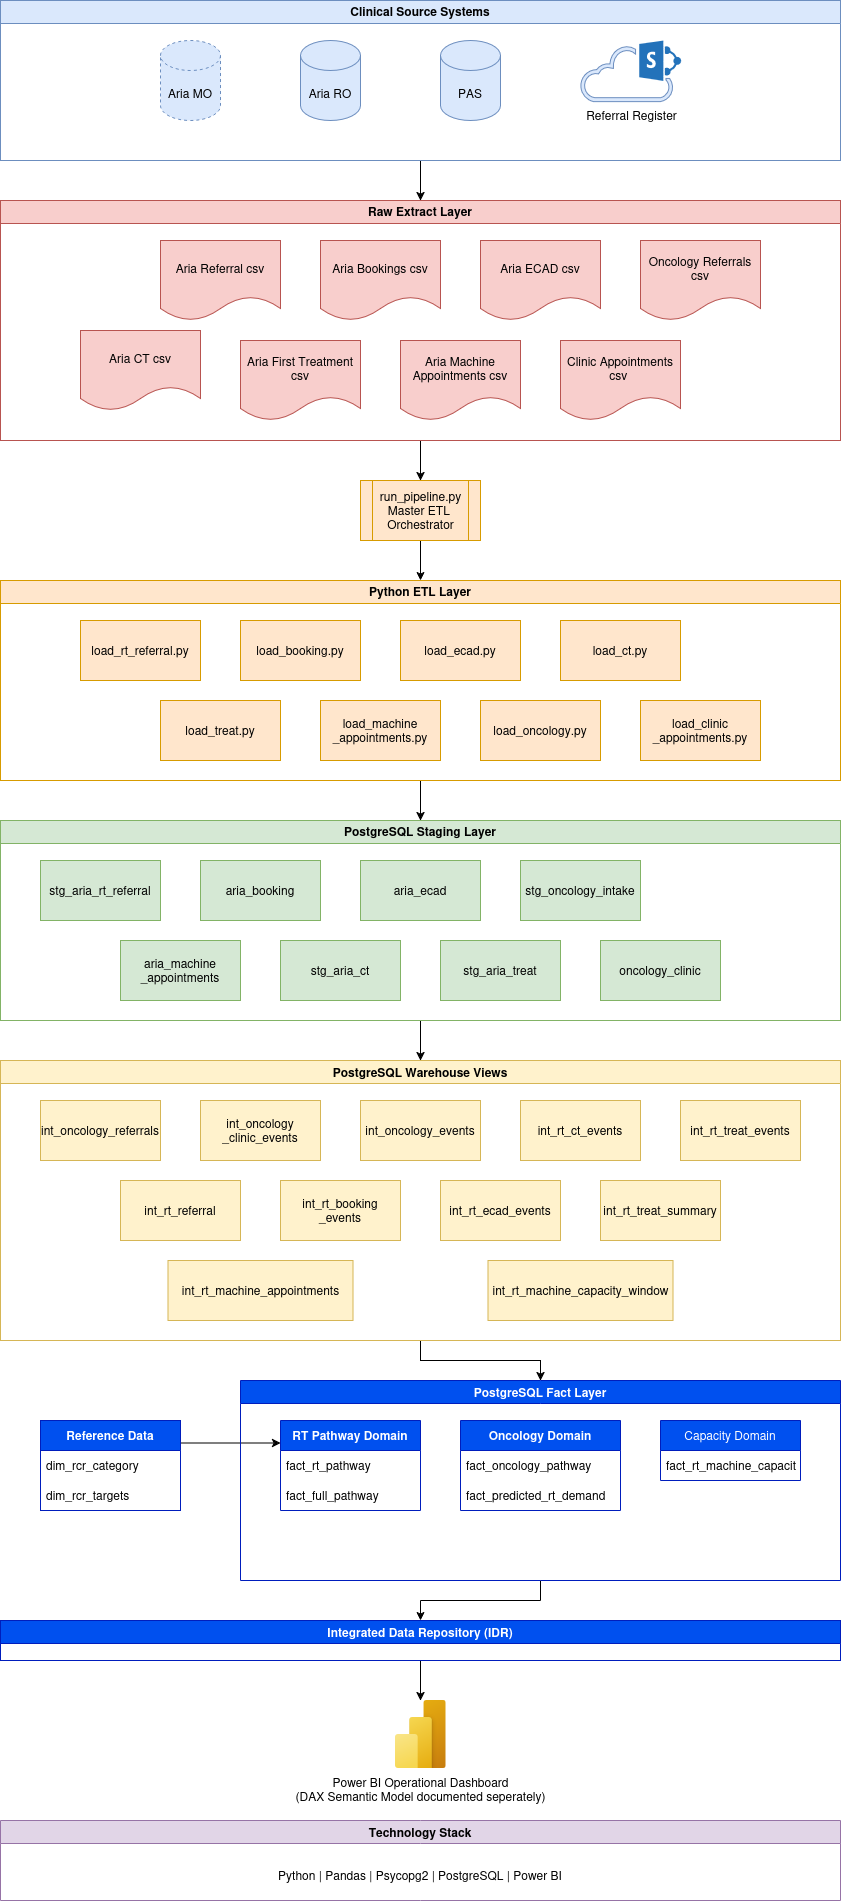
\includegraphics[width=0.5\linewidth]{LogicalArchitecture.png}
    \caption{Logical Architecture of the Integrated Data Repository}
    \label{fig:LogicalArch}
\end{figure}

\subsubsection{Software Engineering and Operational Design}

Although the artefact was developed as a research prototype, several software-engineering practices were incorporated to improve reliability and maintainability.

Logging was implemented throughout the ETL process to support monitoring, troubleshooting, and auditability. All major extractions, transformation and loading activities produced structured log entries allowing operational issues to be investigated retrospectively.

Database credentials and configuration settings were externalised through environment variables rather than being embedded directly within the application code. This approach aligns with principles outlined within the Twelve-Factor App methodology, seperating configuration from code and reducing the risk of credential exposure. 

Togetherm these practices improved operational robustness and facilitated deployment accross development and production environments without modification to application source code. 


\subsection{Pathway Data Model}

\begin{figure}
    \centering
    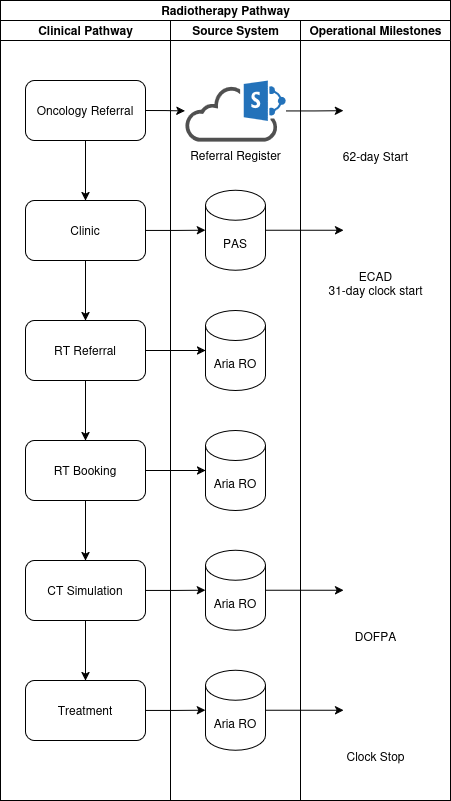
\includegraphics[width=0.5\linewidth]{RTPathwayDataLineage.png}
    \caption{Radiotherapy Pathway, Source Systems and Performance Milestones}
    \label{fig:RTpath}
\end{figure}

The purpose of the pathway data model was to transform fragmented operational records into a series of standardised pathway events capable of supporting interval analysis. A key challenge identified during development was individual source systems recorded only portions of the over all oncology pathway. Consequently, no single source provided a complete end-to-end view from referral to treatment initiation. 

The pathway model therefore adopted a canonical event-based approach. Individual operational events were mapped to a common set of pathway milestones including referral receipt, oncology triage, first clinic appointment, radiotherapy referral, CT simulation, and treatment commencement. These events were subsequently linked through patient identifiers and temporal matching logic to create an integrated representation of each patient pathway. 

From these canonical events, a series of operational intervals were derived, including referral-to-triage, triage-to-clinic, clinic-to-radiotherapy referral, radiotherapy referral-to-CT simulation, and CT simulation-to-treatment. These intervals formed the basis of all dashboard metrics and pathway analyses. 

The use of standardised pathway events aligned with Design Principle 3, ensuring that all metrics were derived consistently across source systems and remained traceable to their originating records. Figure \ref{fig:RTpath} illustrates the relationship between pathway events, source systems, and derived performance milestones.

\subsubsection{Dashboard Development}

Three operational dashboards were developed using Microsoft Power BI. Each dashboard was designed to support a distinct operational management task while sharing a common data repository and data model. 

The Oncology Referrals dashboard focused on referral management activities and provided visibility of active referrals, clinic waiting times, booking lead times, and unresolved clinic outcomes. The dashboard combined referral-register data with clinic activity to provide a current operational view of patients progressing through the oncology pathway. 

The Radiotherapy Service Health dashboard focused on treatment delivery and capacity management. Operational metrics included active patients, expected future referrals, booking backlog, patient risk categorisation, and projected capacity utilisation. Particular emphasis was placed on presenting risk information alongside capacity and demand metrics to support operational intervention. 

The Post-MDT Pathway Overview dashboard integrated data from both oncology and radiotherapy workflows to provide an end-to-end view of patient progression from referral to treatment. The dashboard visualised pathway intervals, operational bottlenecks, and trends in pathway performance over time. 

A fourth dashboard addressing Systemic Anti-Cancer Therapy (SACT) pathways was identified during requirements elicitation. However, due to the lack of a reliable and stable SACT data source during the study period, this component was deferred for future development.

\subsubsection{Iterative Artefact Refinement}
Artefact development followed an iterative process consistent with Design Science Research principles. Successive prototypes were demonstrated to operational stakeholders, with feedback being incorporated into later design iterations. 

The first development cycle focused on radiotherapy operational management. Initial prototypes concentrated on patient tracking and waiting-time performance; however, stakeholder feedback identified a need for greater visibility of future demand and available treatment capacity. This led to the development of capacity-demand forecasting visuals and booking risk indicators. 

The second development cycle focused on oncology referral management. Early versions primarily reported referral volumes and clinic activity. User feedback indicated a stronger operational requirement for active waiting-list management, prompting the addition of patient-group classifications, current booked waits, and referral worklists prioritised by waiting time. 

The third development cycle focused on integrated pathway analysis. Stakeholders identified a need to understand where delays accumulated across the patient journey rather than within individual operational areas. This resulted in the development of pathway-stage metrics and a cumulative waterfall visual illustrating time spent between referral, triage, clinic attendance, radiotherapy referral, CT simulation, and treatment initiation. 

These iterative refinements ensured that the artefact remained closely aligned with operational requirements while simultaneously providing evidence regarding the effectiveness of the proposed design principles.

\subsubsection{ETL and Data Harmonisation}
Data harmonisation presented a significant challenge due to variation in identifier quality, inconsistent recording practices, and differences in operational workflows between source systems. 

NHS numbers were used as the primary identifier wherever possible and were standardised during transformation to remove formatting inconsistencies. Date formats were similarly harmonised to support accurate interval calculations across systems. 

The oncology referral dataset presented particular challenges because it functioned as an operational activity log rather than a controlled referral register. Multiple records were frequently associated with the same oncology episode, reflecting administrative updates, onward referrals, and pathway exceptions. Intermediate transformation views were therefore developed to consolidate records and create a single analytical representation of each referral episode. 

Additional business rules were implemented to identify external-provider referrals, duplicate records, deferred follow-up appointments, and non-standard pathways. These rules allowed operational reporting to focus on patients actively progressing through the pathway while preserving the underlying source data for audit purposes. 

Following transformation and quality-control activities, analytics-ready fact tables were constructed for oncology pathways, radiotherapy pathways, and integrated referral-to-treatment pathways. These fact tables formed the data source for all dashboard visualisations and performance metrics.

\subsection{Data Quality Management}

Exploratory analysis identified several data-quality challenges including duplicate referral records, delayed administrative updates, missing appointment outcomes, and inconsistent coding practices. Rather than modifying source data directly, data-quality controls were implemented within the transformation layer of the repository. 

Business rules were used to identify duplicate referral episodes, exclude non-standard pathways from operational waiting-time calculations, and classify clinician-directed surveillance appointments separately from active patient pathways. This approach preserved the fidelity of source data while improving the validity and interpretability of analytical outputs. 

Data-quality findings were also treated as a research outcome in their own right, providing insight into the operational limitations of existing pathway-monitoring processes and informing recommendations for future pathway digitisation initiatives.

\section{Design Principles} \label{DP}
Design principles represent the design knowledge contribution of this study. They are formulated using a standard DSR structure: \emph{context, intervention}, and \emph{rationale}. These initial principles are refined following evaluation.

\subsection*{DP1: Surface Breach Risks as a Leading Indicator}
If operational teams must prioritise actions in time-constrained cancer pathways, then dashboards should surface leading indicators of breach risk (e.g. days remaining to breach thresholds), because prospective visibility enables earlier and more effective intervention than retrospective compliance metrics. 

\subsection*{DP2: Pair Risk Information with Actionable Capacity Data}
If users are expected to act on identified risks, then risk indicators should be presented alongside relevant capacity and demand information, because risk awareness without visible operational levers does not support decision-making.

\subsection*{DP3: Use Canonical, Standard-Aligned Pathway Events}
If pathway metrics are to be trusted and comparable, then all intervals should be derived from canonical event definitions aligned to NCWTMDS rules, because inconsistent definitions undermine credibility and evaluation validity. 

\subsection*{DP4: Match Data Refresh Cadence to the Action Horizon}
If decisions depend on short operational windows, then data refresh frequency should be aligned to the decision horizon (e.g. daily or near–real-time where feasible), because stale information degrades decision quality.

\subsection*{DP5: Preserve Data Provenance and Auditability}
If analytics are deployed in regulated healthcare environments, then all derived metrics must maintain transparent provenance to source systems, because trust, governance, and reconciliation are essential for adoption.

\subsection*{DP6: Align Interaction Design with Real Operational Tasks}
If dashboards are intended to support complex operational work, then interaction design should reflect users’ real task sequences, because task-aligned interfaces reduce cognitive load and improve decision quality \citep{internationalorganizationforstandardization2020}.

These principles directly inform both the IDR architecture and the dashboard design, and serve as evaluation criteria in Section \ref{EvalStrat}.

\section{Evaluation Strategy} \label{EvalStrat}

Evaluation combines formative and summative methods across four dimensions.

\subsection{Usability Evaluation}
\begin{itemize}
    \item System Usability Scale (SUS)
    \item Heuristic review grounded in ISO 9241-110
    \item Think-aloud walkthroughs
\end{itemize}

\subsection{Utility and Effectiveness}
\begin{itemize}
    \item Task-based experiment with operational users
    \item Primary measures:
    \begin{itemize}
        \item time-to-answer key operational questions,
        \item accuracy of breach-risk identification,
        \item decision quality in constrained scheduling scenarios
    \end{itemize}
\end{itemize}

\subsection{Technical Validity}
\begin{itemize}
    \item Reconciliation of dashboard metrics with source SQL queries
    \item Validation of interval derivations against NCWTMDS rules
\end{itemize}

\subsection{Design Knowledge Evaluation}
\begin{itemize}
    \item Synthesis of user feedback and performance outcomes
    \item Refinement and confirmation of final design principles
\end{itemize}

\section{Ethical and Governance Considerations}
The study operates within UK GDPR and NHS data governance requirements. All data are de-identified or pseudonymised, with access controls and separation between operational and research use. The project follows university ethics procedures and local Trust information governance guidance.

\subsection{Research Limitations}

\begin{itemize}
    \item \textbf{Single-site study:} The artefact will be developed and evaluated within a single NHS Trust, which may limit generalisability.
    \item \textbf{Data quality and availability:} Findings depend on the completeness and accuracy of source systems.
    \item \textbf{Retrospective data:} Restrospective data may not fully represent future operational conditions.
    \item \textbf{Usability sample size:} Evaluation participants are likely to represent a relatively small operational user population. 
    \item \textbf{Artificial evaluation environment:} Demonstration scenarios may not fully replicate live decision-making environments.
    \item \textbf{DSR limitation:} Evaluation assesses utility and usability rather than directly measuring improvements in patient outcomes.
\end{itemize}
\section{Summary}
This chapter has outlined a rigorous, design-science-based methodology that supports both artefact creation and theory-driven knowledge contribution. By embedding explicit design principles within the DSR framework and evaluating the artefact using multiple complementary methods, the study ensures methodological robustness, practical relevance, and academic contribution.

\chapter{Results and Analysis}\label{results}
\section{Introduction}
This chapter presents the results obtained from the development and application of the Integrated Data Repository (IDR) and decision-support dashboard suite described in Chapter \ref{method}. Following construction of the repository, integrated pathway data were analysed to identify operational bottlenecks, assess service demand and capacity, and evaluate the utility of the artefact for supporting operational decision-making. 

Findings are presented according to the research objectives. The chapter begins by summarising repository development and data quality findings before presenting analysis of oncology referrals, radiotherapy operational performance, and end-to-end pathway delays. The chapter concludes by examining the extent to which the developed artefact supports the design principles established in Chapter \ref{method}.

\section{Repository Development Results}
The IDR successfully integrated datasets originating from multiple operational systems including oncology referral register, Patient Administration System (PAS), and the Aria radiotherapy management system. Data were extracted, transformed and loaded into a PostgreSQL-based repository using layered architecture consisting of staging, intermediate and analytical reporting layers. 

Development of the repository identified several previously unrecognised data quality and interoperability challenges. These included duplicate oncology referral records, inconsistent representation of referral episodes, delayed administrative updates, and differences in event definitions between operational systems. 

The use of intermediate integration views allowed business rules to be applied without modifying source data directly. This approach enabled the construction of analytics-ready fact tables capable of supporting operational reporting while preserving auditability and traceability to originating systems. 

The repository subsequently became the single source of truth for all dashboard metrics and pathway analysis. 

\section{Oncology Referral Analysis}

\subsection{Referral Workload}
 Figure \ref{fig:DB_Onc} presents the Oncology Referral Dashboard developed to support management of referral workload, appointment access, and clinic outcome recording. 

 \begin{figure}[htbp]
    \centering
    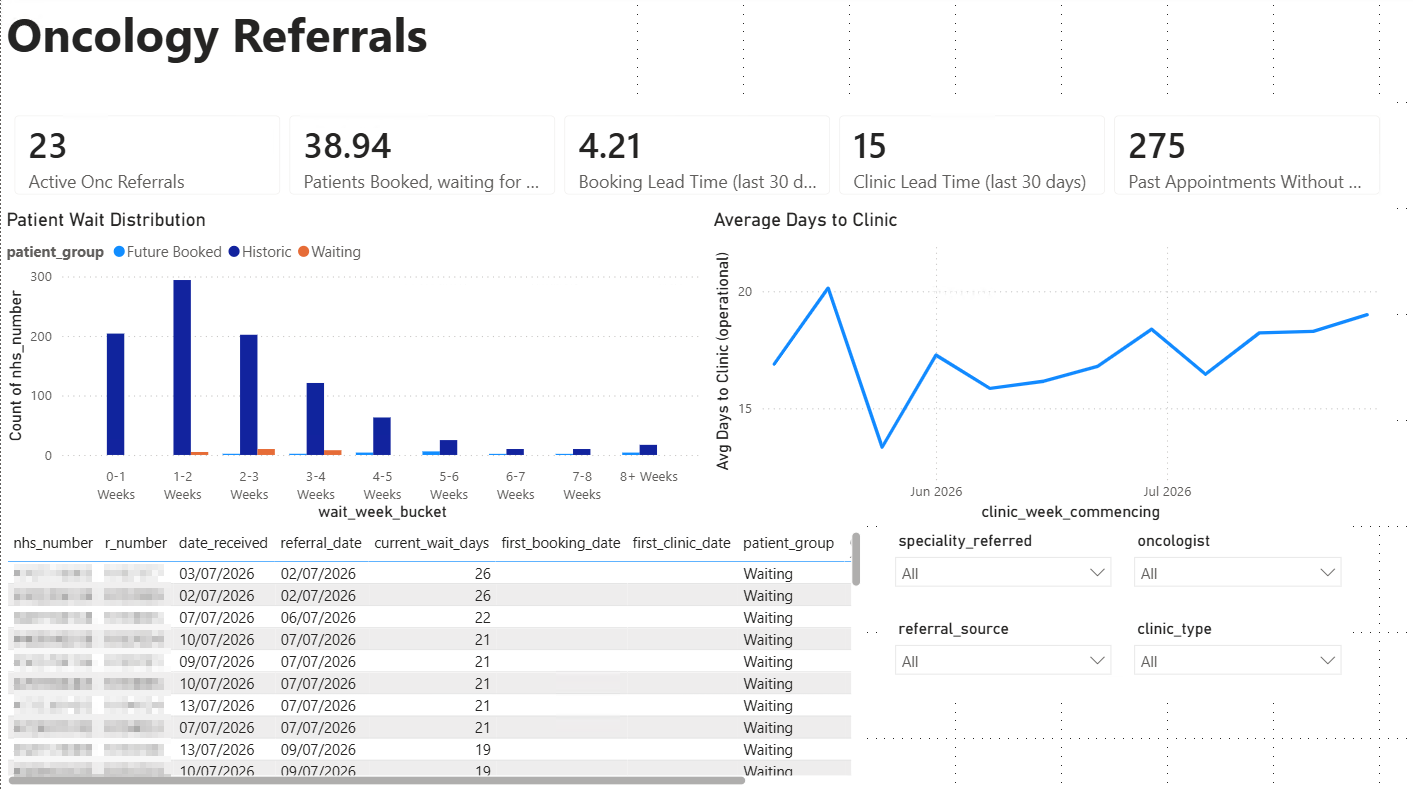
\includegraphics[width=0.85\textwidth]{DB_Onc.png}
    \caption{Operational Oncology Referral Dashboard}
    \label{fig:DB_Onc}
\end{figure}

 Analysis of the oncology referral dashboard identified 23 active oncology referrals at the time of analysis. While this represents a manageable operational workload, variation was observed in waiting times between referral and clinic attendance. 

The distribution of patient waits demonstrated that the majority of patients were clustered within the first three weeks following referral. Smaller numbers of patients remained on the waiting list beyond six weeks, suggesting that the majority of referrals progressed through the booking process relatively efficiently.

\subsection{Booking and Clinic Lead Times}
The average referral-to-booking interval during the previous 30 days was 4.15 days, indicating that referrals were generally triaged and allocated appointments within one working week.

The median referral-to-clinic interval was 15 days. Trend analysis demonstrated that this value remained relatively stable across the observation period, fluctuating between approximately 13 and 20 days.

These findings suggest that initial referral processing and appointment allocation were not the primary sources of pathway delay. The majority of patients received clinic appointments within a timeframe considerably shorter than national cancer waiting-time thresholds.

\subsection{Future Booked Waits}
Patients holding future clinic appointments had an average booked waiting time of 38.94 days. 

This metric should be interpreted carefully, as it does not represent patients awaiting their first oncology appointment following referral. First-appointment access is more accurately reflected by the referral-to-clinic interval, which remained stable at a median of 15 days. 

The future booked wait metric incorporates a broader range of appointment types including routine follow-up appointments, treatment reviews, surveillance activity, and result-discussion clinics. Consequently, the longer waiting time observed is likely to reflect the scheduling characteristics of ongoing oncology care rather than delays affecting newly referred patients. 

Nevertheless, the measure provides useful visibility of future clinic workload and demonstrates demand already committed within existing clinic schedules. This information may assist operational planning by highlighting the volume of future activity competing for available clinic capacity.

\subsection{Incomplete Outcome Recording}
The dashboard identified 275 historical clinic appointments without recorded outcomes. 

This finding represents a significant data-quality issue because pathway progression, attendance analysis, and downstream performance reporting depend upon accurate recording of appointment outcomes. The presence of a large number of unresolved appointments highlights the importance of integrated operational monitoring and demonstrates how the artefact can reveal process weaknesses that may not be visible through conventional reporting. 

\section{Radiotherapy Service Analysis}


\subsection{Operational Workload}

Figure \ref{fig:DB_RT} illustrates the Radiotherapy Service Health Dashboard developed to support monitoring of utilisation, demand forecasting, and patient risk status.

\begin{figure}[htbp]
    \centering
    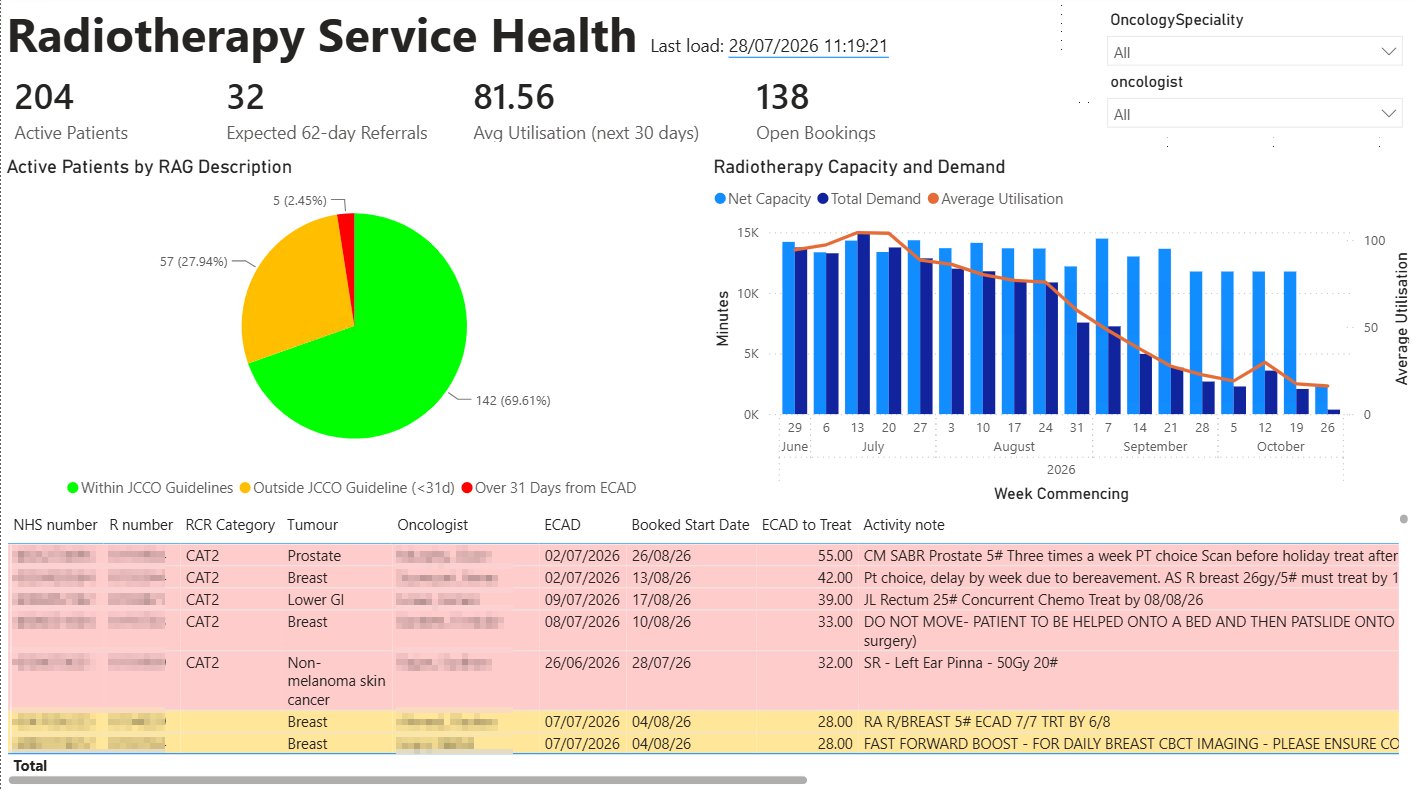
\includegraphics[width=0.85\textwidth]{DB_RT.png}
    \caption{Radiotherapy Capacity and Demand Dashboard}
    \label{fig:DB_RT}
\end{figure}

The radiotherapy dashboard identified 204 active patients undergoing management within the radiotherapy pathway.

In addition, 32 future referrals were predicted to enter the service under a 62-day pathway, defined as oncology referrals booked into Clinical Oncology clinic. This provides operational managers with advance visibility of future demand and supports proactive planning of treatment capacity. 

\subsection{Capacity Utilisation}
Capacity-demand modelling identified an average projected utilisation of 81.56\% across the next 30 days, exceeding the departmental planning threshold of 80\%. This threshold is used operationally to preserve flexibility for urgent treatments, machine downtime, replanning activity, and other unplanned service pressures.

Forecast utilisation declined across the later periods of the planning horizon. However, this reduction should be interpreted with caution because future demand is inherently less complete than near-term demand. The model includes patients currently booked for treatment and referrals that have already entered the radiotherapy pathway, but does not yet reflect patients who have not progressed sufficiently through upstream stages of the pathway. Consequently, the later forecasting periods are likely to underestimate true future demand. 

Despite this limitation, the model provides a useful indication of current service pressure and demonstrates that the radiotherapy service is operating at or slightly above its internal planning threshold.

\subsection{Patient Risk Stratification}
Patient-level risk analysis identified: 

\begin{itemize}
    \item 142 patients (69.61\%) within JCCO guidelines \citep{ash2004}.
    \item 57 patients (27.94\%) outside JCCO guidelines, but within NCWT targets \citep{johnson2024}.
    \item 5 patients (2.45\%) outside the NCWT 31-day standard.
\end{itemize}

Although the majority of patients remained within the recommended timeframes, the presence of patients approaching or exceeding target thresholds demonstrates the value of a proactive monitoring approach.

Rather than identifying breaches retrospectively, the dashboard allows operational teams to focus attention on patients most likely to experience future delays. 

\section{End-to-End Pathway Analysis}


\subsection{Pathway Duration}

Figure \ref{fig:DB_Over} presents the integrated pathway dashboard, combining referral, clinic, and radiotherapy data to visualise pathway progression and identify bottlenecks.

\begin{figure}[htbp]
    \centering
    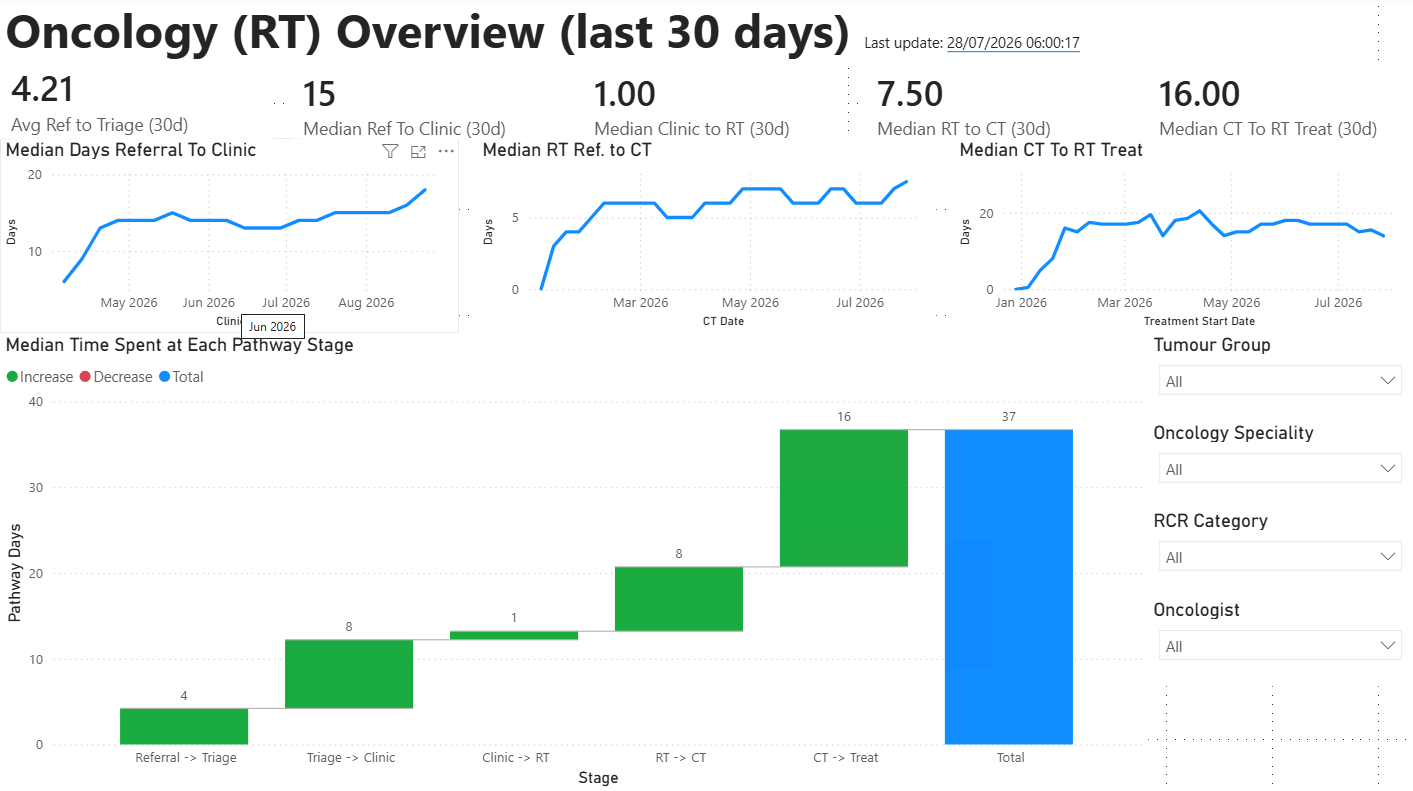
\includegraphics[width=0.85\textwidth]{DB_Overview.png}
    \caption{Integrated Post-MDT Pathway Dashboard}
    \label{fig:DB_Over}
\end{figure}

The integrated pathway dashboard (Figure \ref{fig:DB_Over}) enabled analysis of patient progression from referral through to treatment initiation.

The median pathway duration was 37 days and was composed of five principal operational stages:

\begin{table}[h]
    \centering
    \begin{tabular}{|p{7.5cm}|p{7.5cm}|}
        \hline
        \textbf{Stage} & \textbf{Days} \\
        \hline\hline
        Referral \textrightarrow Triage & 4 \\
        Triage \textrightarrow Clinic & 8 \\
        Clinic \textrightarrow RT Referral & 1 \\
        RT Referral \textrightarrow CT & 8 \\
        CT \textrightarrow Treatment & 16 \\
        \hline
        \textbf{Total} & \textbf{37} \\
        \hline
    \end{tabular}
    \caption{Median duration between canonical events in the Radiotherapy post-MDT pathway}
    \label{tab:path_dur}
\end{table}

\subsection{Bottleneck Identification}
The cumulative waterfall visual shown in Figure \ref{fig:DB_Over} demonstrates the largest delay occurred between CT simulation and treatment commencement, accounting for 16 days of the overall pathway.

The second-largest delay occurred between triage and first clinic attendance, accounting for 8 days.

Together these two stages represented approximately two-thirds of the total pathway duration, suggesting that operational improvement efforts should be concentrated in these areas.

In contrast, the interval between clinic attendance and radiotherapy referral was only one day, indicating that MDT and consultant decision-making processes were not a significant source of delay.

\subsection{Temporal Trends}
Trend analysis demonstrated that:

\begin{itemize}
    \item Referral-to-clinic performance remained relatively stable.
    \item RT Referral-to-CT increased from approximately 0 days to 7 days before stabilising.
    \item CT-to-Treatment remained consistently between 15 and 20 days.
\end{itemize}

The persistence of the CT-to-treatment interval suggests that a substantial proportion of pathway time is spent between CT simulation and treatment initiation. However, this interval represents an aggregation of several planning and preparation activities rather than a single operational process. 

Following CT simulation, patients typically undergo contouring, treatment planning, plan review, quality assurance, and treatment scheduling before treatment can commence. These activities do not currently form part of the canonical pathway events recorded within the repository but nevertheless consume operational time and resources. 

Consequently, further investigation is required before this interval can be interpreted solely as a treatment-capacity issue. Opportunities for future work are discussed in Chapter \ref{discussion}.

\subsection{Research Question 1}
The pathway dashboard directly addressed Research Question 1:

\textbf{Where do delays occur between MDT outcome and treatment?}

Analysis demonstrated that delays are concentrated primarily within:

\begin{enumerate}
    \item CT Simulation \textrightarrow Treatment Start.
    \item Triage \textrightarrow Clinic Attendance.
\end{enumerate}

These stages therefore represent the most significant opportunities for operational intervention. 

\section{Evaluation of Design Principles}

\begin{table}[h]
    \centering
    \begin{tabular}{|p{7.5cm}|p{7.5cm}|}
        \hline
        \textbf{Design Principle} & \textbf{Evidence from Artefact} \\
        \hline\hline
        DP1: Surface Breach Risks & RAG categorisation and patient risk worklists \\
        DP2: Pair Risk with Capacity & Capacity and demand dashboard visualisations \\
        DP3: Canonical Events & Standardised pathway intervals derived from warehouse fact tables \\
        DP4: Refresh Cadence & Automated ETL pipeline and scheduled refresh processes \\
        DP5: Provenance and Auditability & Staging, intermediate and fact-layer architecture with ETL logging \\
        DP6: Task-Oriented Design & Separate referral, radiotherapy and pathway dashboards aligned to operational workflows \\
        \hline
    \end{tabular}
    \caption{Artefact evidence of Design Principles}
    \label{tab:DP-Art}
\end{table}

The evaluation suggests that all six design principles were successfully implemented within the final artefact.

Particularly strong support was observed for DP1 and DP2. Operational users were able to identify patients approaching target breaches while simultaneously assessing available capacity to address identified risks. This combination moved reporting from retrospective performance measurement towards proactive operational management.

\section{Summary}
The developed IDR successfully integrated multiple operational datasets and enabled detailed analysis of post-MDT oncology workflows. Repository development exposed several data quality challenges while establishing a unified analytical platform for operational decision support.

Analysis of oncology referrals demonstrated relatively efficient referral processing while also highlighting the importance of distinguishing first-appointment activity from ongoing follow-up workload.

End-to-end pathway analysis demonstrated that the greatest delays occur between CT simulation and treatment initiation, with an additional contribution arising between triage and first clinic attendance. These findings provide evidence-based targets for future service improvement initiatives and demonstrate the practical utility of the developed artefact for operational oncology management.
\chapter{Discussion and Conclusions}\label{discussion}
\section{Introduction}
This chapter discusses the findings presented in Chapter \ref{results} in relation to the research objectives, literature review, and design principles developed through the Design Science Research process. The chapter evaluates the extent to which the artefact addressed the identified problem, reflects upon the strengths and limitations of the solution, and considers opportunities for future development.

\section{Discussion of Research Question 1}
\textbf{Where do delays occur between MDT outcome and treatment?}

The primary objective of this study was to improve visibility of delays occurring between MDT outcome and treatment initiation. Analysis of the integrated pathway demonstrated that delays were not distributed evenly across the pathway. Rather, two stages accounted for the majority of elapsed time: triage-to-clinic attendance (8 days) and CT simulation-to-treatment initiation (16 days). 

The triage-to-clinic interval represents a period during which referrals are reviewed, prioritised, booked, and ultimately seen by an oncologist. Although the observed interval remained well within national cancer waiting time standards, it nevertheless represented a meaningful proportion of the overall pathway duration. This finding suggests that clinic access capacity remains an important determinant of pathway flow and warrants continued operational monitoring. 

The CT simulation-to-treatment interval represented the largest component of the pathway. However, unlike other pathway stages, this interval does not correspond to a single operational activity. Instead, it encompasses multiple planning processes including target contouring, treatment planning, peer review, quality assurance activities, and treatment booking. Consequently, the current analysis identifies where time accumulates but cannot yet determine which individual planning activities contribute most significantly to delay. 

These findings support the argument presented within the literature that aggregated treatment interval metrics provide limited understanding of operational bottlenecks. By decomposing the pathway into canonical events, the artefact provided substantially greater visibility than traditional compliance reporting.

\section{Discussion of Research Question 2}
\textbf{What operational factors are associated with delay?}

A secondary objective of this study was to identify operational factors associated with delay. Although the repository was not designed as a predictive modelling platform, several factors emerged during analysis. 

First, increasing future clinic waits were observed despite relatively short historic referral-to-clinic intervals. Patients holding future appointments were waiting substantially longer than patients who had already completed the clinic stage. Although future booked waits were considerably longer than the referral-to-clinic interval, these waits largely reflected planned follow-up and review activity rather than new-patient access. The finding therefore provides greater insight into future clinic workload than referral-processing performance. Further investigation, incorporating clinic templates and appointment-type classifications, would be required before conclusions could be drawn regarding clinic-capacity constraints affecting new referrals.

Second, data-quality issues emerged as an operational factor in their own right. A substantial number of clinic appointments lacked recorded outcomes, while duplicate referral records and inconsistent pathway representations required extensive harmonisation during ETL processing. These findings indicate that administrative recording practices can influence both operational visibility and service-management effectiveness. 

Third, radiotherapy demand was observed to operate close to departmental planning thresholds. Although utilisation remained within operationally manageable levels, average projected utilisation exceeded the internal planning threshold of 80\%. This finding highlights the importance of balancing efficiency with sufficient flexibility to accommodate urgent treatments and unplanned events.

\section{Artefact Evaluation}
The artefact successfully achieved its primary objective of providing integrated operational visibility across previously disconnected stages of the post-MDT oncology pathway. 

From a technical perspective, the repository successfully integrated data from multiple heterogeneous operational systems using a common ETL framework. Automated refresh processes reduced manual data processing requirements while preserving data provenance and auditability. 

From an operational perspective, the dashboard suite provided users with visibility of referral activity, clinic performance, radiotherapy capacity, and end-to-end pathway progression. The separation of functionality across multiple dashboards appeared to support task-focused operational workflows without overwhelming users with excessive information. 

Importantly, the development process demonstrated that substantial value can be obtained from relatively lightweight integration architectures. Rather than replacing existing systems, the artefact created a unified analytical layer across existing operational data sources.

\section{Evaluation of Design Principles}
The Design Principles developed in Chapter \ref{method} were intended to represent transferable knowledge extending beyond the specific implementation used in this study. 

DP1 and DP2 received particularly strong support during evaluation. Risk-based patient categorisation and capacity-demand visualisation enabled operational users to identify not only where delays existed but also whether sufficient operational capacity existed to mitigate those risks. 

DP3 was supported through the use of canonical pathway events aligned to published cancer waiting time standards. The pathway model enabled consistent interval calculation across multiple source systems and reduced ambiguity associated with locally defined metrics. 

DP4 was partially supported. While daily automated refreshes were achieved for the majority of datasets, dependency upon external operational reports limited refresh frequency for some clinic data extracts. Nevertheless, the data remained sufficiently current to support operational decision-making. 

DP5 was supported through the separation of staging, transformation, and reporting layers, allowing all reported metrics to be traced back to source records. 

DP6 was supported through iterative stakeholder engagement and the creation of task-oriented dashboards aligned with referral management, radiotherapy service management, and pathway performance monitoring respectively. 

Collectively, the evaluation suggests that all six design principles remain valid and may have applicability beyond the specific organisational setting studied.

\section{Reflections and Lessons Learned}
Several important lessons emerged during the development process. 

The most significant lesson related to data quality. Initial assumptions suggested that the primary challenge would involve technical integration of multiple systems. In practice, the greater challenge involved understanding operational processes and interpreting inconsistently recorded data. 

The project also highlighted the value of Design Science Research for healthcare informatics projects. The iterative nature of the methodology enabled technical development to remain aligned with operational requirements while simultaneously generating transferable design knowledge. 

Finally, the study reinforced the importance of stakeholder engagement. Several dashboard features and pathway metrics evolved considerably following operational feedback. This iterative refinement improved both the utility and relevance of the final artefact.

\section{Limitations}

Several limitations should be considered when interpreting the findings. 

First, the study was conducted within a single NHS organisation and therefore reflects local processes, systems, and operational practices. 

Second, the repository relies upon the quality and completeness of source-system data. Although significant harmonisation and validation activities were undertaken, residual inaccuracies within source datasets may still influence results. 

Third, the CT simulation-to-treatment interval represents an aggregation of multiple planning and operational activities. While the repository successfully identifies this stage as a significant contributor to overall pathway duration, the current data model cannot determine precisely how time is distributed between individual planning processes. 

Finally, evaluation focused primarily on operational utility and usability rather than direct patient outcomes. Consequently, although the artefact provides improved operational visibility, the extent to which it contributes to improved clinical outcomes remains outside the scope of the present study.

\section{Future Work}
\subsection{Clinic Capacity Modelling}
Future development should incorporate clinic-capacity modelling and appointment-type classification to better understand demand distribution across new-patient, follow-up, and review clinics. This would provide greater visibility of capacity utilisation and allow more detailed investigation of factors influencing access to first oncology appointments.

\subsection{Digital Referral Forms}

The project identified several data-quality issues attributable to manually maintained processes and retrospective transcription of referral information. Future work should investigate the implementation of structured digital referral forms containing standardised mandatory fields and validation rules. Such an approach may improve data quality while reducing ETL complexity.

\subsection{CT-to-Treatment Decomposition}
The current pathway model treats CT simulation-to-treatment as a single interval. Future repository development should introduce additional canonical events representing contouring, treatment planning, peer review, quality assurance, and treatment booking activities. This would provide a more granular understanding of where delays occur within the treatment-planning process.

\subsection{SACT Integration}
A key future enhancement involves integration of Systemic Anti-Cancer Therapy (SACT) data following completion of the planned Cancer Network-wide system upgrade. Incorporating SACT treatment events would enable end-to-end analysis of all major treatment modalities and provide a more comprehensive representation of post-MDT oncology pathways.

\subsection{Predictive Analytics}
The repository architecture also provides a foundation for future predictive analytics. Potential applications include forecasting breach risk, modelling future demand, and identifying patients likely to experience pathway delays before breaches occur.

\section{Conclusion}
This study has demonstrated that meaningful operational insight can be generated through the integration of existing oncology datasets within a lightweight Integrated Data Repository. Using a Design Science Research methodology, the project successfully developed and evaluated an artefact capable of improving visibility of post-MDT pathway performance. 

The repository identified that delays are concentrated primarily within the triage-to-clinic and CT simulation-to-treatment stages of the pathway. Furthermore, the project demonstrated that significant operational value can be achieved through relatively modest data integration and analytics capabilities without requiring replacement of existing clinical systems. 

Beyond the artefact itself, the study contributes a set of evaluated design principles for operational oncology analytics that may be transferable to other healthcare organisations facing similar challenges relating to fragmented data and pathway visibility. 

The findings therefore contribute both practical value for operational cancer services and academic value through the generation of reusable design knowledge for healthcare informatics.

\clearpage
\addcontentsline{toc}{chapter}{References}
\bibliography{./Project}

\clearpage

\appendix
\chapter{Integrated Data Repository Architecture}\label{appendix:architecture} 
\section{Repository Layers} 

The Integrated Data Repository (IDR) adopted a layered architecture consisting of source systems, staging tables, intermediate integration views, analytical fact tables, and reporting dashboards. This design separated raw operational data from analytical representations while maintaining data provenance and traceability. 

\section{Primary Repository Components} 

\begin{table}[h] 
    \centering 
    \begin{tabular}{|p{4cm}|p{8cm}|} 
        \hline 
        \textbf{Component} & \textbf{Purpose} \\ 
        \hline 
        Staging Layer & Preservation of raw source extracts and audit trail. \\ 
        \hline 
        Integration Layer & Application of business rules and data harmonisation processes. \\
        \hline 
        Fact Tables & Analytics-ready datasets used for operational reporting. \\ 
        \hline 
        Power BI Layer & Operational dashboards and data visualisation. \\ 
        \hline 
    \end{tabular} 
    \caption{Repository Architecture Components} 
\end{table} 

\section{Source Systems} 

\begin{table}[h] 
    \centering 
    \begin{tabular}{|p{3cm}|p{4cm}|p{5cm}|} 
        \hline 
        \textbf{Source} & \textbf{Data Type} & \textbf{Purpose} \\ 
        \hline 
        Oncology Referral Register & SharePoint List & Oncology referral management \\ 
        \hline Patient Administration System (PAS) & Operational Reports & Clinic bookings and attendance \\ 
        \hline 
        Aria OIS & CSV Extracts & Radiotherapy referral, CT and treatment activity \\ 
        \hline 
    \end{tabular} 
    \caption{Primary Data Sources} 
\end{table} 

\section{Logical Architecture} 

Figure \ref{fig:LogicalArch} in Chapter \ref{method} illustrates the logical architecture of the repository.
\chapter{Data Dictionary}\label{appendix:datadictionary}

\begin{table}[H]
    \centering
    \begin{tabular}{|p{5cm}|p{8cm}|} 
        \hline
        \textbf{Column} & \textbf{Description} \\ 
        \hline 
        oncology\_referral\_date & Date oncology referral received. \\ 
        \hline
        oncology\_booking\_date & Date first oncology appointment booked \\ 
        \hline 
        oncology\_clinic\_date & Date first oncology clinic attended. \\ 
        \hline 
        rt\_referral\_date & Date referral received by radiotherapy service. \\ 
        \hline 
        ecad\_referral\_date & Earliest clinically agreed decision-to-treat date. \\ 
        \hline 
        ct\_date & CT simulation date. \\ 
        \hline 
        first\_completed\_treat\_date & First completed radiotherapy fraction. \\ 
        \hline 
        days\_onc\_to\_clinic & Days from referral to first oncology clinic. \\ 
        \hline 
        days\_rt\_to\_ct & Days from radiotherapy referral to CT simulation. \\ 
        \hline 
        days\_ct\_to\_treat & Days from CT simulation to treatment start. \\ 
        \hline 
        operational\_risk\_group & Current operational risk classification. \\ 
        \hline 
        booking\_rag\_status & Booking risk category. \\ 
        \hline 
    \end{tabular}
    \caption{Data Dictionary}
\end{table}
\chapter{Example ETL and Business Rules}\label{appendix:etl}

\section{Identifier Standardisation}
NHS numbers were standardised during transformation to remove formatting inconsistencies and improve matching across source systems. 

\begin{verbatim} 
    REPLACE(nhs_number,' ','') 
\end{verbatim}

\section{Referral Consolidation Logic} 

The oncology referral register contained multiple administrative records relating to individual referral episodes. Intermediate integration views consolidated these records into a single analytical representation. 

\begin{verbatim} 
    Multiple referral updates 
    ↓ 
    Business-rule consolidation 
    ↓ 
    Single referral episode 
\end{verbatim}

\section{Radiotherapy Pathway Status Classification} 

\begin{verbatim} 
    CASE 
        WHEN has_completed = 1 THEN 'Treated' 
        WHEN has_cancelled = 1 THEN 'Closed - Cancelled' 
        WHEN has_active_booking = 1 THEN 'Active' 
        WHEN booking_completed_date IS NOT NULL 
            THEN 'Closed - No Treatment' 
        ELSE 'Awaiting Booking' 
    END 
\end{verbatim}

\section{Canonical Pathway Events} 

The repository transformed operational events into standardised pathway milestones: 

\begin{enumerate} 
    \item Referral Received 
    \item Oncology Triage 
    \item First Oncology Clinic 
    \item Radiotherapy Referral 
    \item CT Simulation 
    \item Treatment Commencement 
\end{enumerate} 

These events provided the basis for interval calculations and pathway analysis.
\chapter{Dashboard Evaluation Results} \label{appendix:evaluation} 

\section{Participants} 
Three operational stakeholders participated in the evaluation of the dashboard suite. 

\begin{table}[h] 
    \centering 
    \begin{tabular}{|p{3cm}|p{8cm}|} 
        \hline 
        \textbf{Participant} & \textbf{Role} \\ 
        \hline\hline
        P1 & Clinical Oncology Director \\ 
        P2 & Radiotherapy Operations Manager \\ 
        P3 & Lead Treatment Radiographer \\ 
        \hline 
    \end{tabular} 
    \caption{Evaluation Participants} 
\end{table}

\section{System Usability Scale Results} 
\begin{table}[h] 
    \centering 
    \begin{tabular}{|l|c|} 
        \hline 
        \textbf{Participant} & \textbf{SUS Score} \\ 
        \hline\hline 
        P1 & 95.0 \\ 
        P2 & 90.0 \\ 
        P3 & 95.0 \\ 
        \hline 
        Mean & 93.3 \\ 
        \hline 
    \end{tabular} 
    \caption{System Usability Scale (SUS) Results} 
\end{table} 

The dashboard suite achieved a mean SUS score of 93.3, indicating a very high level of perceived usability.

\section{Operational Value Assessment} 

Participants rated the following statements using a five-point Likert scale (1 = Strongly Disagree, 5 = Strongly Agree). 

\begin{table}[h] 
    \centering 
    \begin{tabular}{|p{9cm}|c|} 
        \hline 
        \textbf{Statement} & \textbf{Mean Score} \\
        \hline\hline
        The dashboard improves visibility of post-MDT pathway performance & 5.0 \\
        The dashboard helps identify patients at risk of target breaches & 5.0 \\ 
        Displaying capacity and demand information supports operational decision-making & 4.7 \\ 
        The dashboard reduces reliance on manual reporting processes & 5.0 \\ 
        I would incorporate this dashboard into routine operational management activities & 4.7 \\ 
        \hline 
    \end{tabular} 
    \caption{Operational Value Assessment} 
\end{table}


\section{Design Principle Validation} 

\begin{table}[H]
    \centering 
    \begin{tabular}{|p{9cm}|c|} 
        \hline 
        \textbf{Statement} & \textbf{Mean Score} \\ 
        \hline\hline
        The dashboard helps identify risks before breaches occur & 5.0 \\ 
        Capacity information is presented in a useful and actionable way & 5.0 \\ 
        The pathway stages reflect meaningful operational events & 4.7 \\ 
        Information is refreshed frequently enough for operational use & 4.3 \\ 
        I trust the dashboard metrics & 4.0 \\ 
        The dashboard supports my day-to-day operational tasks & 4.3 \\ 
        \hline 
    \end{tabular} 
    \caption{Design Principle Evaluation Results} 
\end{table}
\clearpage
\section{Qualitative Feedback} 
\begin{table}[h] 
    \centering 
    \begin{tabular}{|p{4cm}|p{10cm}|} 
        \hline 
        \textbf{Theme} & \textbf{Feedback} \\ 
        \hline\hline
        Most Useful Features & Waterfall visualisation of pathway delays; filtering by oncologist and speciality; patient worklists and breach monitoring. \\ 
        Missing Information & SACT data; clinic utilisation; visibility of emergency inpatient referrals to radiotherapy; utilisation breakdown by machine availability versus service demand. \\ 
        Operational Decisions Supported & Referral monitoring; patient tracking; bottleneck identification; overtime planning; shift extensions; additional linear accelerator capacity; capacity planning based on expected referrals. \\
        Future Enhancements & Clinic-capacity modelling; CT-to-treatment decomposition; utilisation analysis; integration of structured electronic referrals and SACT datasets. \\ 
        General Comments & ``Very good. Can't wait to start using it.'' \newline ``Looks good.'' \newline Electronic referral implementation was identified as a useful future data source for before-and-after evaluation studies. \\ 
        \hline 
    \end{tabular} 
    \caption{Summary of Qualitative Feedback} 
\end{table}
\end{document}
    
